\documentclass{oblivoir}

\usepackage[utf8]{inputenc}
\usepackage{setspace}
\usepackage{amsmath}
\usepackage{parskip}
\usepackage{amsfonts}
\usepackage{amssymb}
\usepackage{mathtools}
\usepackage{xlop}
\usepackage{graphicx}
\graphicspath{ {./images/} }
\usepackage{bold-extra}
\usepackage{rotating}
\setlength{\parskip}{5pt}
\setlength{\parindent}{0pt}
\usepackage[colorlinks]{hyperref}
\usepackage{caption}
\usepackage{xcolor}



\newcommand{\hs}{\hspace*{3mm}}
\newcommand{\hhs}{\hspace*{6mm}}
\newcommand{\hhhs}{\hspace*{14.45mm}}
\newcommand{\vs}{\vspace*{1mm}}

\usepackage{geometry}
 \geometry{
 a4paper,
 total={170mm,257mm},
 left=30mm,
 right=30mm,
 top=30mm,
 bottom=45mm
 }
 

\title{\vspace{-1cm}C++ Exercise \\ \huge{Neural Network for MNIST}}
\author{Hyeon Jeon \\ \small{\href{hj@hcil.snu.ac.kr}{hj@hcil.snu.ac.kr}}}
\date{}
\usepackage{natbib}
\usepackage{graphicx}

\begin{document}
\setstretch{1.1}

\maketitle
\vspace{-1cm}
\section{Introduction}


In this exercise, you will implement a basic neural network consists of 3 layers, which classifies handwritten digits provided by the MNIST dataset. By the exercise, you will understand the following concepts:
\begin{itemize}
    \item Class and inheritance in cpp
    \item How neural network \& backpropagation works
\end{itemize}

\section{Background}

\subsection{MNIST dataset} 

MNIST(Modified National Institute of Standards and Technology database) dataset is a large database of handwritten digits, which is widely used for training and testing image processing systems based on deep learning / machine learning models. Since 1998, lots of computer scientists tried to implement AI, which can classify the images, and recently the researchers from the University of Virginia announced the model, which achieved 99.82\% accuracy.

\begin{figure}[h]
    \centering
    \includegraphics{images/mnist.png}
    {\caption*{MNIST dataset}}
\end{figure}

MNIST contains 60,000 training images and 10,000 test images, and they're provided in \texttt{mnist} directory. Also, 
accessing and reading files is already implemented; hence you only need to focus on implementing a neural network that receives the data from MNIST as input. 

\subsection{Brief History}

In the early stage of AI(Artificial Intelligence), it was mostly rule-based. Researchers extracted the patterns from data and tried to encode them as rules heuristically. However, the strategy was quite not successful, as it was hard to obtain every underlying pattern from data. 

On the other hand, in the 1970-80s, several researchers, including Geoffrey Hinton, David Rumelhart, Yoshua Bengio, tried another approach: Artificial neural network. Their approach mainly aimed to mimic the neuron \& synapse structure of the human brain. However, due to its high computation requirement, the approach was extremely inefficient and was discarded for decades; we now call this era as \textit{AI winter}.

However, as the computation power had come a long way, the time and resource usage for Artificial Neural Network decreased significantly, and it showed overwhelming performance. Moreover, as now researchers can collect unlimited data from the internet, it got the opportunity to be adopted in various domains. Therefore, nowadays, AI became one of the most important modern technologies, and learning AI \& neural networks is now an essential course for researchers in the engineering or science field. 

\subsection{Perceptron}

Perceptron is an algorithm offered by Frank Rosenblatt in 1957 and now used as a fundamental element in many complex neural networks. The structure is quite simple: it combines several inputs and generates single output. 
\begin{figure}[h]
    \centering
    \includegraphics[height=5cm]{images/perceptron.png}
    {\caption*{Single perceptron}}
\end{figure}

The $y$ value is determined like this: 
\begin{align*}
    y = 1 \text{ if } x_1w_1 + x_2y_2 + x_3y_3 > \theta \\
    y = 0 \text{ if } x_1w_1 + x_2y_2 + x_3y_3 < \theta
\end{align*}


where $\theta$ is a threshold. However, a single-layer perceptron can only classify the space linearly; it cannot be applied to the complex non-linear situation. To solve the problem, researchers constructed a neural network as a sophisticated multi-layer perceptron. 
\begin{figure}[h]
    \centering
    \includegraphics[height=5cm]{images/percep_linear.png}
    {\caption*{Linear vs. Nonlinear perceptron \\ \scriptsize{(Reference: https://jtsulliv.github.io/perceptron/)}}}
\end{figure}

In this exercise, you'll implement a multi-layer perceptron. For the detailed explanation for our neural network, refer next section.

\section{Explanation}

\subsection{Neural network}

As I mentioned above, our neural network will consist of 3 layers: input, hidden, and output, which are \textit{fully connected}. The structure overview and specification for each part are as follows.

\begin{figure}[h]
    \centering
    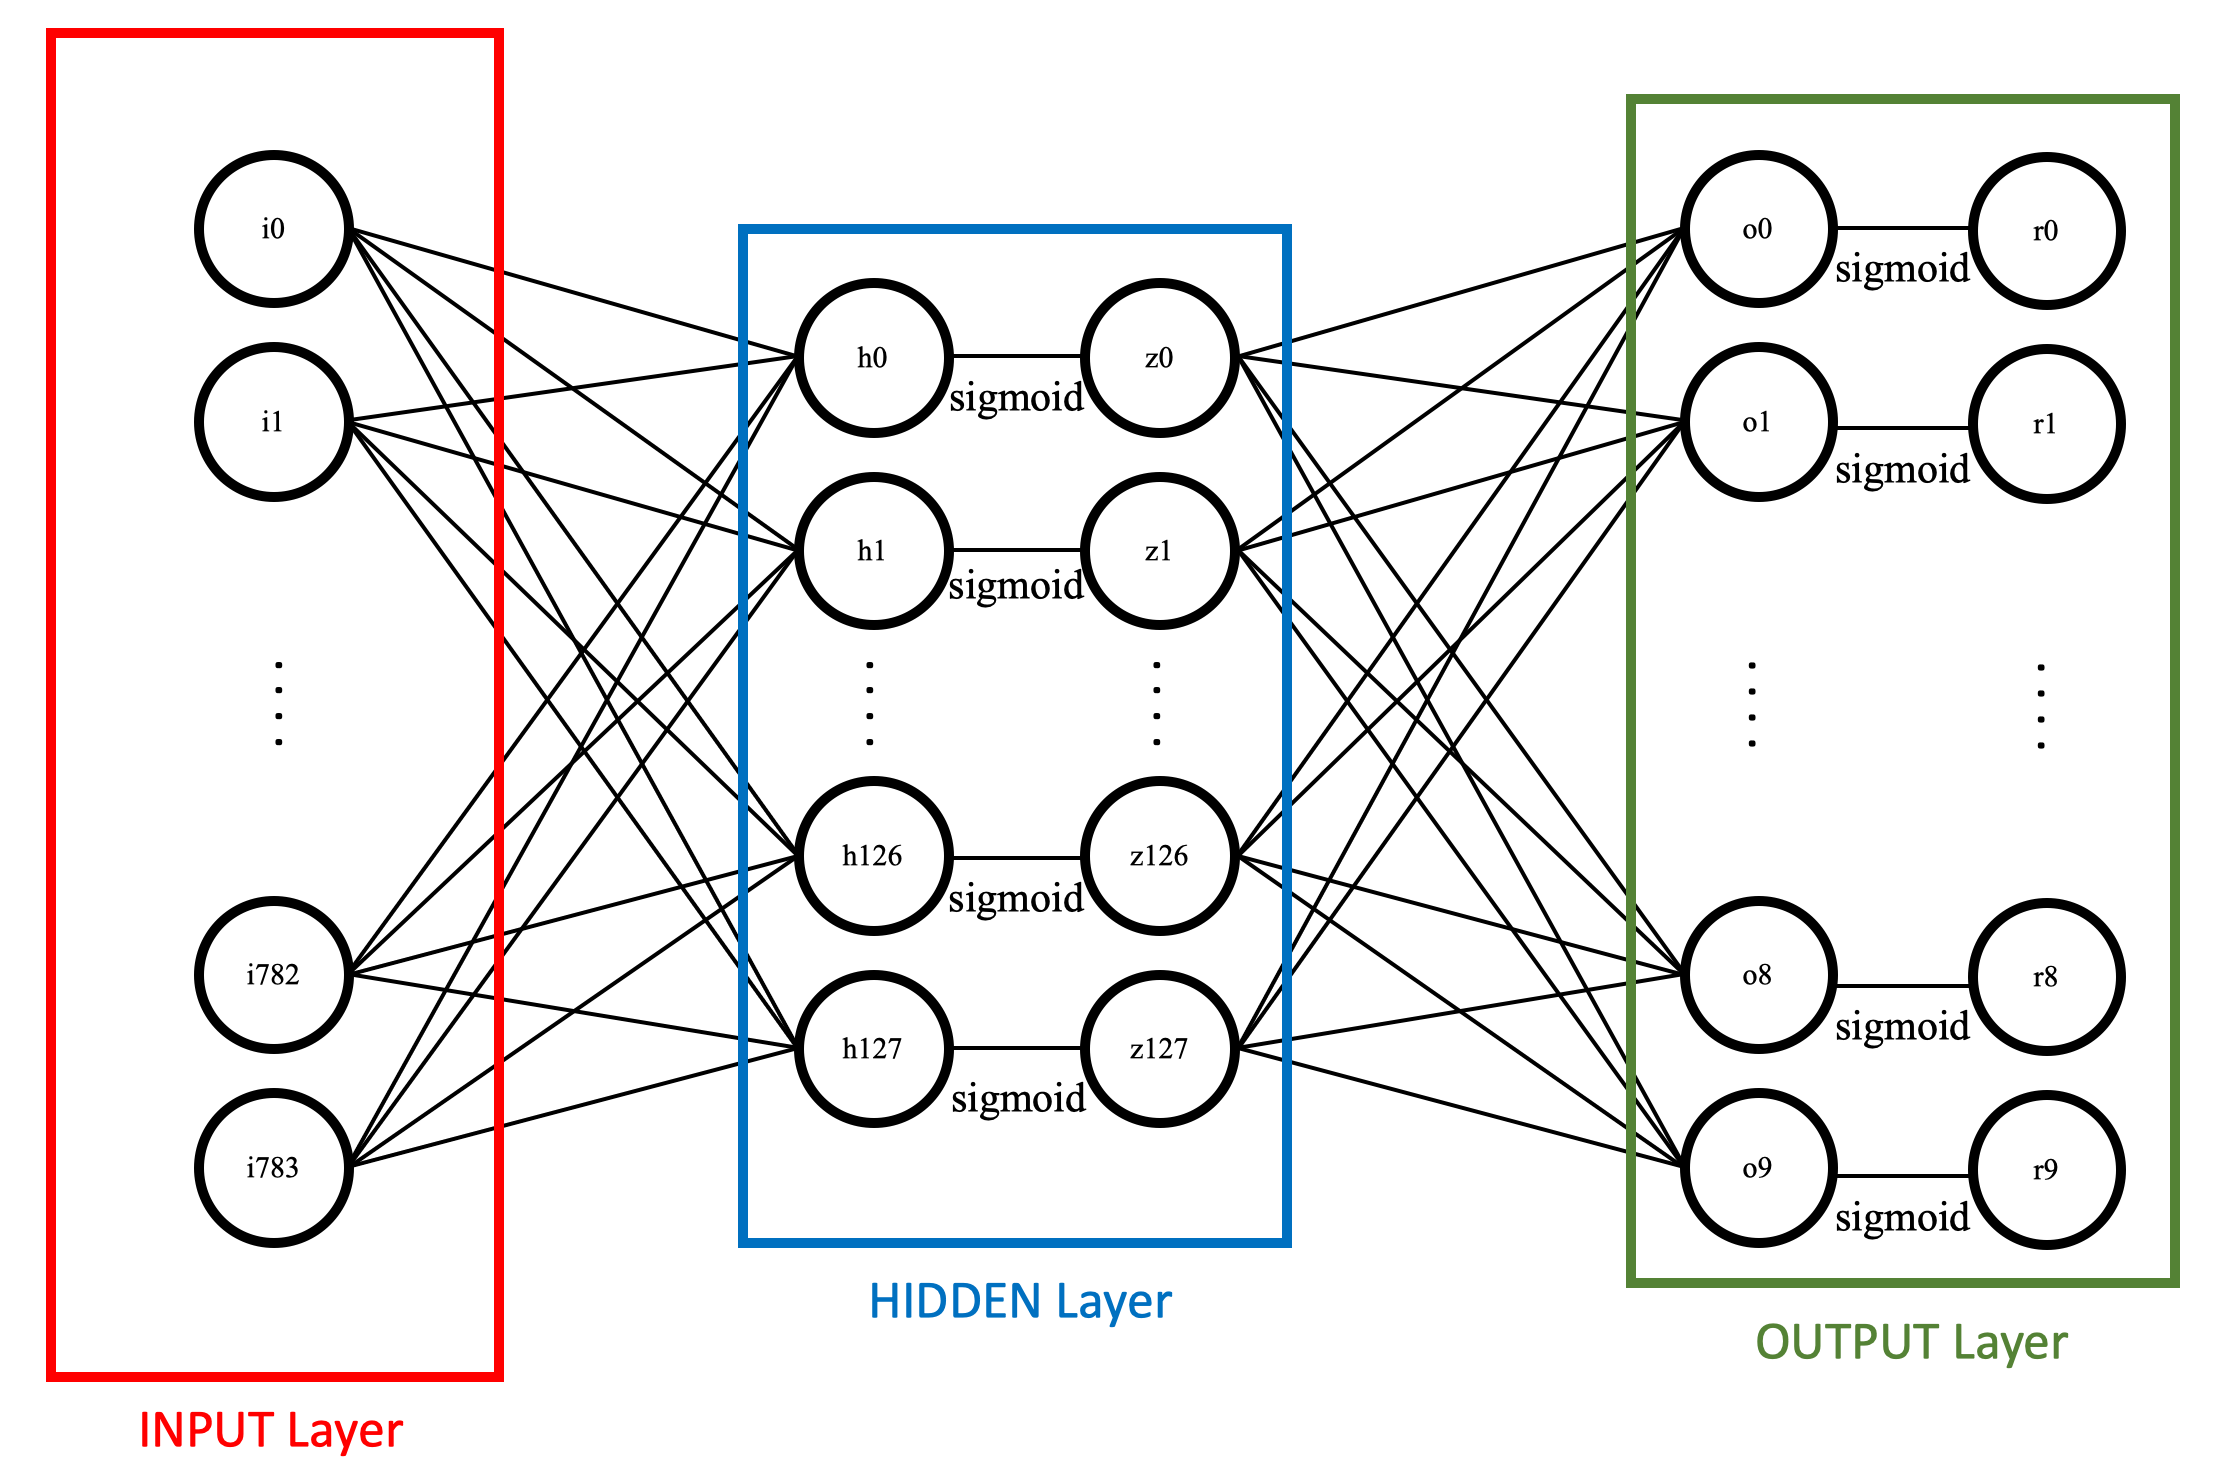
\includegraphics[height=8cm]{images/overview.png}
    {\caption*{Neural network structure overview}}
\end{figure}

As the MNIST image size is $28 \times 28 = 784$, There are total 784 nodes in the input layer. The hidden layer initially has 128 nodes, but you can modify it freely. Last, the output layer has ten nodes, where each represents the corresponding digit (0-9). 

\subsection{Activation function}

You might notice that both the hidden layer and the output layer have a single edge named \textit{Sigmoid}. It is an \textit{Activation function} for our neural network. So what is activation function? To understand the activation function, you must recall that the single-layer perceptron generates linear classification, and a multi-layer approach had arrived to solve the problem. However, if we overlap multiple linear perceptrons successively, it still produces linear classification. A simple example might help you: overlapping $y=ax$ and $z=by$ just generates $z = b \cdot ax$, which is still linear.

Therefore, a non-linear function should be located between linear perceptrons, and the activation function serves the role. There exist various modern non-linear activation functions: ReLU, Leaky ReLU, tanh, Softmax, Swish.... 

Activation function has one more important property: it controls the power of the signal. Let's remind that the basic perceptron generates only two kinds of signal: 0 to 1 (transfer or not). However, researchers found that transferring the signal value is more effective in solving complex problems. But to transfer continuous value, the output of the perceptron should be post-processed to maintain consistency. The activation function helps the neural network to achieve the goal. For instance, Sigmoid normalizes the input value to a value between 0 and 1. 

\subsubsection{Sigmoid}

Sigmoid, or logistic regression, which you'll implement, is quite an old strategy. The function and its graph are like this:
\begin{align*}
    \text{Sigmoid}(x) = \frac{e^x}{1 + e^x}
\end{align*}
\begin{figure}[h]
    \centering
    \includegraphics[height=5cm]{images/sigmoid_graph.png}
\end{figure}

As represented in the graph, Sigmoid sends a large positive number to 1 and the opposite to -1. Sigmoid has some critical problems: exponential function inside it requires high computation, and sometimes immensely slows down the training.  Nevertheless, it is easy to implement and also fits our problem. You'll notice the benefit of Sigmoid in \textbf{backpropagation section}.  

\subsection{Training}

The training step of typical neural networks, including our network, follows the process: 
\begin{enumerate}
    \item Get current input
    \item Perform feed-forward computation through the network
    \item Calculate Loss
    \item Backpropagate the loss and update weights
    \item Go back to step 1 with next input
\end{enumerate}

Let's see the detail with our neural network.

\subsubsection{Feed-Forward}

Our network starts with the connection between the Input layer and the Hidden layer.

\begin{figure}[h]
    \centering
    \includegraphics[height=7cm]{images/input_hidden.png}
\end{figure}

Let's denote each input value(node) as $I_i$ and hidden layer input value as $H_i$. Then the overall computation across Input and Hidden layer is as follows:
\begin{align*}
    H_i = W_{0, i}I_0 + W_{1, i}I_1 + \cdots + W_{782, i}I_{782} + W_{783, i}I_{783} + b_i
\end{align*}
where $i$: 0 to 127 (128 hidden nodes), $W_{a,b}$ corresponds to the edge connecting $I_a$ and $H_b$, and $b_i$ denotes the bias. 

Hidden layer also contains Sigmoid. Let's denote Sigmoid as $\phi$ and it's result as $Z_i$. Then we can just say $\phi(H_i) = Z_i$ where $i$: 0 to 127.

Now only the connection between Hidden / Output layer and the final Sigmoid are left. These computations are like this:
\begin{align*}
    O_i &= W'_{0, i}Z_0 + W'_{1, i}Z_1 + \cdots + W'_{126, i}Z_{126} + W'_{127, i}Z_{127} + b'_i & \\
    R_i &= \phi(O_i) & i: 0 \text{ to } 9
\end{align*}
where $O_i$: Output layer input value, and $R_i$: Final result value.


\subsubsection{Loss function}

As final result $R_i$s are the output of Sigmoid, their value is in between zero and one. Next step is to calculate loss. In this exercise, you'll implement \textit{MSE(Mean Squared Error)}:
\begin{align*}
    MSE = \frac{1}{2}\Sigma_{i=0}^{9}(\hat{R}_i - R_i)^2 \\
    \hat{R}_i = 0 \text{ if } label == i \text{ else } 0 
\end{align*}
as loss function, where $\hat{R}_i$ denotes the real result. The value of real result vector $\hat{R}$ is defined as above. For example, if the input image represents digit 7, $\hat{R}$ will be $(0,0,0,0,0,0,0,1,0,0)$.

Therefore, if our neural network assigns a high value to the index corresponds to the answer and low value to the others, the loss will be small. Therefore, we interpret the final result value vector of $R$ as follows: $\text{answer} = \arg\max R_i$.
\subsubsection{Backpropagation}
Now we learned how our neural network generates the answer and the way to calculate the loss. Then, how can we \textit{train} our neural network? Backpropagation, which was first suggested by Rumelhart et al. in their \href{https://www.iro.umontreal.ca/~vincentp/ift3395/lectures/backprop_old.pdf}{\textcolor{blue}{paper}} published in \textit{Nature}, provides a polished way to achieve the goal. 

The main concept of backpropagation is to send back the generated loss(or error) toward the input and underlying weights. While sending back the error, the gradient for each weight will be calculated successively, and the weights will be updated due to their gradients. So how can we calculate gradient \textit{successively}? The theoretical background for this step is quite simple: \textit{chain rule}.

Maybe you had learned partial derivative and chain rule in the calculus class. For who did not or who forgot the concepts, I'll briefly explain them. The former is quite a straightforward concept: a partial derivative of a function of several variables is its derivative concerning one of those variables, with the others held constant. For example, partial derivative ${\partial f}/{\partial x}$ of the function $f(x,y) = ax^2 + bxy + cy^2$ will be:
\begin{align*}
    \frac{\partial f}{\partial x} = 2ax + by.
\end{align*}
This is the only thing you need to know about partial derivative. 

Then how about chain rule? Astonishingly, you had noticed the basic concept of the chain rule in high school. Recall the famous derivative rule $(f(g(x))' = f'(g(x)) \cdot g'(x)$, which can be written as
\begin{align*}
     \frac{df \circ g}{dx} = \frac{df}{dg} \cdot \frac{dg}{dx}
\end{align*}
by the Leibniz's notational system. This directly shows the main idea of the chain rule: the derivative can be calculated through the consecutive sequence of inner derivatives. A simple example will help you. Let's think about the composite function $f(g(h(i(x))))$. The derivative of the function can be calculated through the sequence:
\begin{align*}
    (f(g(h(i(x)))))' &= f'(g(h(i(x)))) \cdot (g(h(i(x))))' \\
                     &= f'(g(h(i(x)))) \cdot g'(h(i(x))) \cdot (h(i(x)))' \\
                     &= f'(g(h(i(x)))) \cdot g'(h(i(x))) \cdot h'(i(x)) \cdot i'(x)
\end{align*}
which can be expressed as 
\begin{align*}
    \frac{df}{dx} = \frac{df}{dg} \cdot \frac{dg}{dh} \cdot \frac{dh}{di} \cdot \frac{di}{dx},
\end{align*}
which is the standard form of the chain rule. Of course, chain rule can be applied to partial derivative too.

Then how can we apply these concepts to update weights during backpropagation? The main purpose of the backpropagation is to reduce the loss. And our error, MSE, can be expressed as the function of variables $W, b, I$, where each denotes the set of weight, bias, and input values. Therefore, it is evident that we can calculate the partial derivative of MSE due to each weight and bias, and the value can be evaluated using the chain rule. After calculating the gradient, the weight can be updated toward the direction, which reduces the loss. The equation below explains the work.
\begin{align*}
    w = w - \eta \frac{\partial MSE}{\partial w}
\end{align*}
In the equation, $w$ denotes a certain weight, and $\eta$ is the learning rate. If the learning rate is low, the training's precision will become high, but it will take much time to arrive at the point. In contrast, a high learning rate will ensure both fast training and low precision. 

\begin{figure}[h]
    \centering
    \includegraphics[height=5cm]{images/gradient.png}
    \caption*{Weight update due to its gradient}
\end{figure}

Now its time to follow the backpropagation step. Let's first recall the entire feed-forward process. 

\begin{align*}
     H_i &= W_{0, i}I_0 + W_{1, i}I_1 + \cdots + W_{782, i}I_{782} + W_{783, i}I_{783} + b_i & \\
     Z_i &= \phi(H_i) & i: 0 \text{ to } 127 \\
     O_j &= W'_{0, j}Z_0 + W'_{1, j}Z_1 + \cdots + W'_{126, j}Z_{126} + W'_{127, j}Z_{127} + b_j' & \\
     R_j &= \phi(O_j) & j: 0 \text{ to } 9 \\
     MSE &= \frac{1}{2}\Sigma_{k=0}^{9}(\hat{R}_k - R_k)^2 &
    \hat{R}_k = 0 \text{ if } label == k \text{ else } 0
\end{align*}

The parameters that should be updated are the \textit{weights} and \textit{bias} of the neural network. Let's first investigate $W'_{i,j}$. It is obvious that 
\begin{align*}
    \frac{\partial MSE}{\partial W'_{i,j}} = \frac{\partial MSE}{\partial R_j} \frac{\partial R_j}{\partial O_j} \frac{\partial O_j}{\partial W'_{i, j}},
\end{align*}
and each term of the right-hand side is as follows:
\begin{align*}
    \frac{\partial MSE}{\partial R_j} &= \frac{1}{2} \frac{\partial }{\partial R_j} (\hat{R}_j - R_j)^2  =(\hat{R}_j - R_j) \\
    \frac{\partial R_j}{\partial O_j} &= \frac{\partial\phi(O_j)}{\partial O_j} \\
    \frac{\partial O_j}{\partial W'_{i, j}} &= Z_i
\end{align*}

Now you might ask; "How can we calculate $\frac{\partial\phi(O_j)}{\partial O_j}$" ? Recall that 
\begin{align*}
    \phi(x) = \text{Sigmoid}(x) = \frac{e^x}{1 + e^x} = \frac{1}{1 + e^{-x}}.
\end{align*}
We can easily calculate the derivative using simple derivation rule:
\begin{align*}
    \phi'(x) &= ((1 + e^{-x})^{-1})'  \\ 
    &= (1 + e^{-x})^{-2} \cdot (1 + e^{-x})'  \\
    &= (1 + e^{-x})^{-2} \cdot (-e^{-x}) \\
    &= \frac{1}{1 + e^{-x}} \cdot \frac{-e^{-x}}{1 + e^{-x}} \\
    &= (1 - \phi(x))\phi(x)
\end{align*}
Therefore, we can rewrite the second derivative $\frac{\partial R_j}{\partial O_j}$.
\begin{align*}
    \frac{\partial R_j}{\partial O_j} &= \frac{\partial\phi(O_j)}{\partial O_j} = (1- \phi(O_j))\phi(O_j) = (1-R_j)R_j
\end{align*}

It is easy to notice that $\frac{\partial MSE}{\partial W_{i,j}}$ can be calculated only by using $\hat{R}_j, R_j, Z_i$, which are the values that can be evaluated during the feed-forward step. 

Then How about the bias $b'_j$? We can simply write the gradient like:
\begin{align*}
    \frac{\partial MSE}{\partial b'_j} = \frac{\partial MSE}{\partial R_j} \frac{\partial R_j}{\partial O_j} \frac{\partial O_j}{\partial b'_j},
\end{align*}

Now you might found the issue; we already calculated $\frac{\partial MSE}{\partial R_j}$ and $ \frac{\partial R_j}{\partial O_j}$ while dealing with $W_{i,j}$. Therefore the only thing we need to consider is $\frac{\partial O_j}{\partial b'_j}$, which is 1. 

This fact is one of the most critical points during backpropagation. We can reuse the sequence of partial gradients. The above situation can be illustrated like this. 

\begin{figure}[h]
    \centering
    \includegraphics[width=13cm]{images/backprop.png}
    %\caption*{}
\end{figure}

As we already calculated the gradients corresponding to a green arrow while going toward a red arrow, we don't need to do it again while going toward a blue arrow. This technique reduces computation a lot and therefore accelerates training.

\section{Assignments}

\subsection{Written}

You may be understood how our neural network works. However, I didn't explain everything, so you must first fill up the missing links.

Solve the following problems. It is highly recommended to write the entire process with \LaTeX. 

\begin{enumerate}
    \item In section \textbf{3}, we only calculated the gradients for the second layer. Compute the gradients for the first layer.
    \begin{enumerate}
        \item Compute $\frac{\partial MSE}{\partial W_{i,j}}$.
        \item Compute $\frac{\partial MSE}{\partial b_j}$.
    \end{enumerate}
    \item Recall that our neural network updates the weight by applying
    \begin{align*}
        w = w - \eta \frac{\partial MSE}{\partial w}. 
    \end{align*}
    Prove that this updating strategy ensures the decrease of MSE (\textit{hint: focus on $\Delta MSE$}).
\end{enumerate}

\subsection{Implementation}

The template code is available at the \href{https://jeonhyun97.github.io/cpp_4_undergraduates/cpp/assn/assn3/assn3.zip}{\textcolor{blue}{link}}. The training and testing code are already implemented, so you only need to focus on implementing the feed-forward and backpropagation step. 

The functions that you need to implement is like this:

\begin{itemize}
    \item \texttt{perceptron.cpp}
    \begin{itemize}
        \item \texttt{Perceptron(int num)} \\
        The constructor of a single perceptron, which gets \texttt{num} inputs. Allocate the initial value to the \texttt{num} weights correspond to each input, and a single bias. It is recommended to assign random value to weights / bias using \texttt{rand\_0to1} function in \texttt{helper.cpp}.
        \item \texttt{forward(double* input)} \\
        Feed-forward step for a single perceptron.
        \item \texttt{backprop(double delta, double *current\_input)} \\
        Backpropagation step for a single perceptron. \texttt{delta} denotes the former gradients which are propagated from the fore, and \texttt{current\_input} literally denotes the current input vector for the layer, which contains the perceptron.
    \end{itemize}
    \item \texttt{sigmoid.cpp}
    \begin{itemize}
        \item \texttt{forward(double input)}
        \item \texttt{backprop()}
    \end{itemize}
    \item \texttt{bridge.cpp} \\
    This class represents the bridge between a layer to the other layer. It is consists of the set of perceptrons and sigmoids, according to the input / output structure explained in section \textbf{3.1}. 
    \begin{itemize}
        \item \texttt{Bridge(int input\_num, int output\_num)} \\
        Gets input / output number as arguments, and allocates perceptrons and sigmoids due to the values. 
        \item \texttt{forward(double* input)}
    \end{itemize}
    \item \texttt{hidden\_output.cpp}
    \\ inherites \texttt{Bridge} class, and represents the bridge from the input layer to the hidden layer.
    \begin{itemize}
        \item \texttt{backprop(double* delta)}
    \end{itemize}
    \item \texttt{input\_hidden.cpp}
    \\ inherites \texttt{Bridge} class, and represents the bridge from the input layer to the hidden layer.
    \begin{itemize}
        \item \texttt{backprop(double* delta)} \\
        \texttt{Input\_Hidden :: backprop()} should get the result of \texttt{Hidden\_Output :: backprop()} as a argument.
    \end{itemize}
    \item \texttt{train.cpp}
    \begin{itemize}
        \item \texttt{loss\_function(double* delta)} \\
        \texttt{delta} denotes the array consists of $\hat{R_i} - R_i$, where $i = 0$ to $9$.
    \end{itemize}
\end{itemize}
The area of \texttt{Hidden\_Output} and \texttt{Input\_Hidden} are like this. 

\begin{figure}[h]
    \centering
    \includegraphics[width=12cm]{images/implementation.png}
\end{figure}

After implementation, you can generate executable \texttt{program} by \texttt{make run} command. If the program output is like this, it verifies your implementation.

\begin{figure}[h]
    \centering
    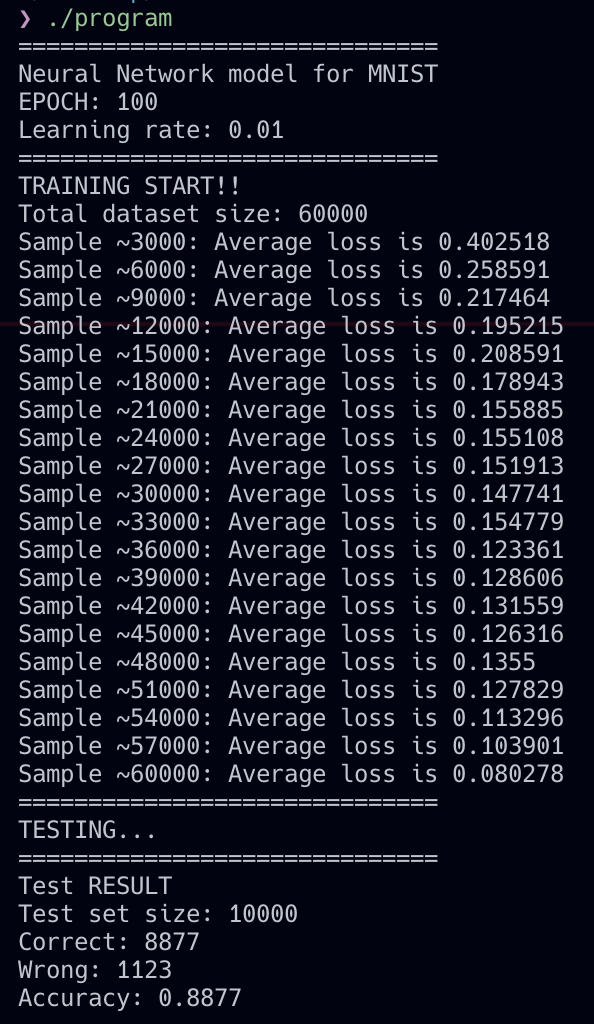
\includegraphics[width=6cm]{images/result.png}
\end{figure}

\subsection{Tips}

\begin{itemize}
    \item Use the constants in \texttt{constants.h}. For fast test \& verification, I recommend you to change the \texttt{EPOCH}
    \item Remember that you only need to implement about \textbf{50} lines. 
\end{itemize}

\end{document}


